\chapter{Joitain polunetsintäalgoritmeja}\label{joitainP}

\section{Leveyssuuntainen läpikäynti (BFS)}\label{bfs}
Leveyssuuntainen läpikäynti, eli leveyshaku (Breadth First Search, BFS) on 
epäinformoitu hakualgoritmi, joka perustuu sokeaan 
hakuun~\cite{applSciLawande}. Siinä graafin solmut ryhmitellään eri tasoihin 
sen mukaan monenko kaaren kautta pitää kulkea lähtösolmusta, jotta niihin 
päästään. Lähtösolmu on tasolla 0, siihen yhdistyneet solmut tasolla 1, 
tason 1 solmuihin yhdistyneet solmut tasolla 2 ja niin edelleen. 
Leveyshaussa graafin kaikki solmut käydään läpi niin, että tarkistetaan 
onko solmussa jo käyty, onko solmu maalisolmu ja mihin solmuihin sillä on 
yhteys. Sitten tallennetaan solmu läpikäytyjen solmujen listalle ja tieto 
siitä, mitä kautta solmulle on tultu~\cite{BFSRahim}. \par
	Ajetaan \textcite{applSciLawande} perusteella 
kirjoitetun, ohjelmalistauksen \ref{BFSEsim} mukaista BFS-algoritmia graafissa 
\ref{refGraf}. Asetetaan lähtösolmuksi G ja maalisolmuksi P. Oletetaan, että 
algoritmille syötetty graafidata on aakkosjärjestyksessä, jonka takia 
algoritmi käy läpi solmuja aakkosten mukaan. Tasoksi 0 asetetaan lähtösolmu G. 
Tason 1 muodostavat siihen yhteydessä olevat solut E, J ja L. Tason 2 soluja 
ovat tason 1 soluissa kiinni olevat solut, eli B, H ja O. Solmua G ei 
huomioida, koska siellä on jo käyty. Joitain solmuja voidaan kuitenkin käydä 
läpi useasti, jos niihin on useampi polku. Algoritmin ajo graafissa 
\ref{refGraf} johtaa kuvan \ref{refBFS} lopputulokseen, jossa on käyty läpi 
syaaninväriset kaaret ja löydetty punaisella merkitty polku G-E-H-K-P. \par
	Ohjelmalistauksen \ref{BFSEsim} algoritmi lopettaa etsinnän 
löydettyään yhden polun, mutta jos algoritmiin ei lisätä tätä lopetusehdoksi, 
niin algoritmi käy läpi kaikki solmut ja kaaret ja löytää kaikki mahdolliset 
polut~\cite{BFSRahim}. Haittapuoliin kuuluu suuri muistinkulutus tallennettujen 
polkujen lukumäärän takia~\cite{BFSRahim}, sekä pitkä 
ajoaika~\cite{mazeGameTrilogi}. Nämä voidaan huomata myös syaaninväristen 
kaarten suuresta määrästä.

\begin{figure}
	\begin{subfigure}[b]{0.3\textwidth}
		\centering
		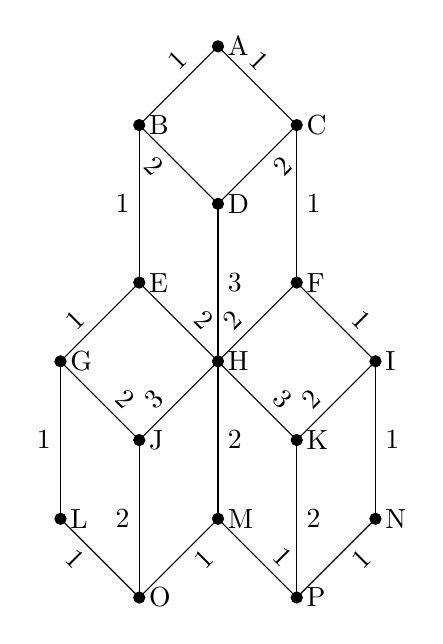
\begin{tikzpicture}[main/.style = {draw, circle}] 
		%Pisteet
		\filldraw[black] (0,6) circle (2pt) node[anchor=west]{A};
		\filldraw[black] (-1,5) circle (2pt) node[anchor=west]{B};
		\filldraw[black] (1,5) circle (2pt) node[anchor=west]{C};
		\filldraw[black] (0,4) circle (2pt) node[anchor=west]{D};
		\filldraw[black] (-1,3) circle (2pt) node[anchor=west]{E};
		\filldraw[black] (1,3) circle (2pt) node[anchor=west]{F};
		\filldraw[black] (-2,2) circle (2pt) node[anchor=west]{G};
		\filldraw[black] (0,2) circle (2pt) node[anchor=west]{H};
		\filldraw[black] (2,2) circle (2pt) node[anchor=west]{I};
		\filldraw[black] (-1,1) circle (2pt) node[anchor=west]{J};
		\filldraw[black] (1,1) circle (2pt) node[anchor=west]{K};
		\filldraw[black] (-2,0) circle (2pt) node[anchor=west]{L};
		\filldraw[black] (0,0) circle (2pt) node[anchor=west]{M};
		\filldraw[black] (2,0) circle (2pt) node[anchor=west]{N};
		\filldraw[black] (-1,-1) circle (2pt) node[anchor=west]{O};
		\filldraw[black] (1,-1) circle (2pt) node[anchor=west]{P};
		% Janat
		\draw (0,6) -- node[midway, above left, sloped] {1} (1,5);	% AB
		\draw (0,6) -- node[midway, above right, sloped] {1} (-1,5);	% AC
		\draw (-1,5) -- node[midway, below left, sloped] {2} (0,4);	% BD
		\draw (-1,5) -- node[midway, left] {1} (-1,3);			% BE
		\draw (1,5) -- node[midway, below right, sloped] {2} (0,4);	% CD
		\draw (1,5) -- node[midway, right] {1} (1,3);			% CF
		\draw (0,4) -- node[midway, right] {3} (0,2);			% DH
		\draw (-1,3) -- node[midway, above left, sloped] {1} (-2,2);	% EG
		\draw (-1,3) -- node[midway, above right, sloped] {2} (0,2);	% EH
		\draw (1,3) -- node[midway, above left, sloped] {2} (0,2);	% FH
		\draw (1,3) -- node[midway, above right, sloped] {1} (2,2);	% FI
		\draw (-2,2) -- node[midway, above right, sloped] {2} (-1,1);	% GJ
		\draw (-2,2) -- node[midway, left] {1} (-2,0);			% GL
		\draw (0,2) -- node[midway, above left, sloped] {3} (-1,1);	% HJ
		\draw (0,2) -- node[midway, above right, sloped] {3} (1,1);	% HK
		\draw (0,2) -- node[midway, right] {2} (0,0);			% HM
		\draw (2,2) -- node[midway, above left, sloped] {2} (1,1);	% IK
		\draw (2,2) -- node[midway, right] {1} (2,0);			% IN
		\draw (-1,1) -- node[midway, left] {2} (-1,-1);			% JO
		\draw (1,1) -- node[midway, right] {2} (1,-1);			% KP
		\draw (-2,0) -- node[midway, below left, sloped] {1} (-1,-1);	% LO
		\draw (0,0) -- node[midway, below right, sloped] {1} (-1,-1);	% MO
		\draw (0,0) -- node[midway, above right, sloped] {1} (1,-1);	% MP
		\draw (2,0) -- node[midway, below right, sloped] {1} (1,-1);	% NP
		\end{tikzpicture}
		\caption{Referenssigraafi.}\label{refGraf}
	\end{subfigure}
	\hfill
	\begin{subfigure}[b]{0.3\textwidth}
		\centering
		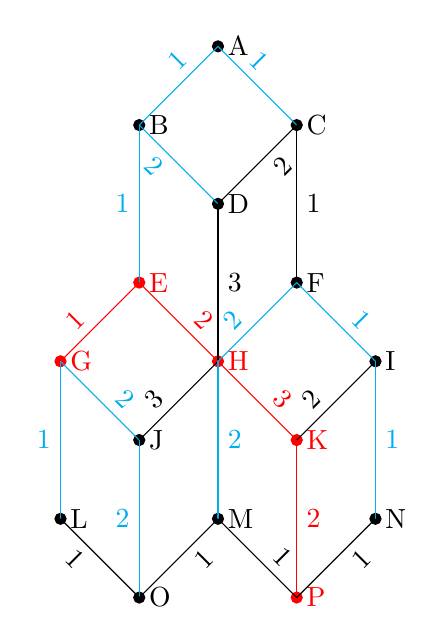
\begin{tikzpicture}[main/.style = {draw, circle}] 
		%Pisteet
		\filldraw[black] (0,6) circle (2pt) node[anchor=west]{A};
		\filldraw[black] (-1,5) circle (2pt) node[anchor=west]{B};
		\filldraw[black] (1,5) circle (2pt) node[anchor=west]{C};
		\filldraw[black] (0,4) circle (2pt) node[anchor=west]{D};
		\filldraw[red] (-1,3) circle (2pt) node[anchor=west]{E};
		\filldraw[black] (1,3) circle (2pt) node[anchor=west]{F};
		\filldraw[red] (-2,2) circle (2pt) node[anchor=west]{G};
		\filldraw[red] (0,2) circle (2pt) node[anchor=west]{H};
		\filldraw[black] (2,2) circle (2pt) node[anchor=west]{I};
		\filldraw[black] (-1,1) circle (2pt) node[anchor=west]{J};
		\filldraw[red] (1,1) circle (2pt) node[anchor=west]{K};
		\filldraw[black] (-2,0) circle (2pt) node[anchor=west]{L};
		\filldraw[black] (0,0) circle (2pt) node[anchor=west]{M};
		\filldraw[black] (2,0) circle (2pt) node[anchor=west]{N};
		\filldraw[black] (-1,-1) circle (2pt) node[anchor=west]{O};
		\filldraw[red] (1,-1) circle (2pt) node[anchor=west]{P};
		% Janat
		\draw [cyan] (0,6) -- node[midway, above left, sloped] {1} (1,5);	% AB
		\draw [cyan] (0,6) -- node[midway, above right, sloped] {1} (-1,5);	% AC
		\draw [cyan] (-1,5) -- node[midway, below left, sloped] {2} (0,4);	% BD
		\draw [cyan] (-1,5) -- node[midway, left] {1} (-1,3);			% BE
		\draw (1,5) -- node[midway, below right, sloped] {2} (0,4);	% CD
		\draw (1,5) -- node[midway, right] {1} (1,3);			% CF
		\draw (0,4) -- node[midway, right] {3} (0,2);			% DH
		\draw [red] (-1,3) -- node[midway, above left, sloped] {1} (-2,2);	% EG
		\draw [red] (-1,3) -- node[midway, above right, sloped] {2} (0,2);	% EH
		\draw [cyan] (1,3) -- node[midway, above left, sloped] {2} (0,2);	% FH
		\draw [cyan] (1,3) -- node[midway, above right, sloped] {1} (2,2);	% FI
		\draw [cyan] (-2,2) -- node[midway, above right, sloped] {2} (-1,1);	% GJ
		\draw [cyan] (-2,2) -- node[midway, left] {1} (-2,0);			% GL
		\draw (0,2) -- node[midway, above left, sloped] {3} (-1,1);	% HJ
		\draw [red] (0,2) -- node[midway, above right, sloped] {3} (1,1);	% HK
		\draw [cyan] (0,2) -- node[midway, right] {2} (0,0);			% HM
		\draw (2,2) -- node[midway, above left, sloped] {2} (1,1);	% IK
		\draw [cyan] (2,2) -- node[midway, right] {1} (2,0);			% IN
		\draw [cyan] (-1,1) -- node[midway, left] {2} (-1,-1);			% JO
		\draw [red] (1,1) -- node[midway, right] {2} (1,-1);			% KP
		\draw (-2,0) -- node[midway, below left, sloped] {1} (-1,-1);	% LO
		\draw (0,0) -- node[midway, below right, sloped] {1} (-1,-1);	% MO
		\draw (0,0) -- node[midway, above right, sloped] {1} (1,-1);	% MP
		\draw (2,0) -- node[midway, below right, sloped] {1} (1,-1);	% NP
		\end{tikzpicture}
		\caption{BFS referenssigraafissa.}\label{refBFS}
	\end{subfigure}
	\hfill
	\begin{subfigure}[b]{0.3\textwidth}
		\centering
		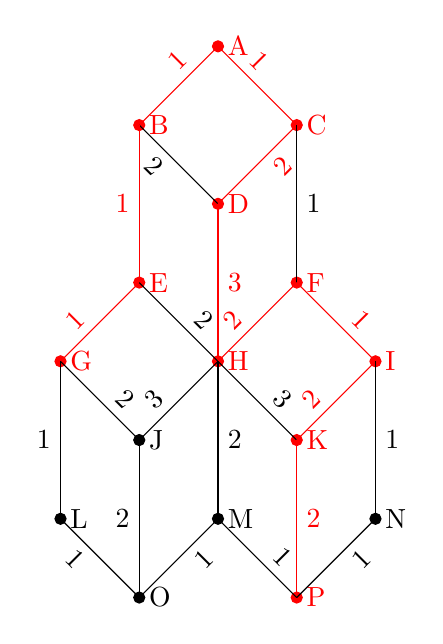
\begin{tikzpicture}[main/.style = {draw, circle}] 
		%Pisteet
		\filldraw[red] (0,6) circle (2pt) node[anchor=west]{A};
		\filldraw[red] (-1,5) circle (2pt) node[anchor=west]{B};
		\filldraw[red] (1,5) circle (2pt) node[anchor=west]{C};
		\filldraw[red] (0,4) circle (2pt) node[anchor=west]{D};
		\filldraw[red] (-1,3) circle (2pt) node[anchor=west]{E};
		\filldraw[red] (1,3) circle (2pt) node[anchor=west]{F};
		\filldraw[red] (-2,2) circle (2pt) node[anchor=west]{G};
		\filldraw[red] (0,2) circle (2pt) node[anchor=west]{H};
		\filldraw[red] (2,2) circle (2pt) node[anchor=west]{I};
		\filldraw[black] (-1,1) circle (2pt) node[anchor=west]{J};
		\filldraw[red] (1,1) circle (2pt) node[anchor=west]{K};
		\filldraw[black] (-2,0) circle (2pt) node[anchor=west]{L};
		\filldraw[black] (0,0) circle (2pt) node[anchor=west]{M};
		\filldraw[black] (2,0) circle (2pt) node[anchor=west]{N};
		\filldraw[black] (-1,-1) circle (2pt) node[anchor=west]{O};
		\filldraw[red] (1,-1) circle (2pt) node[anchor=west]{P};
		% Janat
		\draw [red] (0,6) -- node[midway, above left, sloped] {1} (1,5);	% AB
		\draw [red] (0,6) -- node[midway, above right, sloped] {1} (-1,5);	% AC
		\draw (-1,5) -- node[midway, below left, sloped] {2} (0,4);	% BD
		\draw [red] (-1,5) -- node[midway, left] {1} (-1,3);			% BE
		\draw [red] (1,5) -- node[midway, below right, sloped] {2} (0,4);	% CD
		\draw (1,5) -- node[midway, right] {1} (1,3);			% CF
		\draw [red] (0,4) -- node[midway, right] {3} (0,2);			% DH
		\draw [red] (-1,3) -- node[midway, above left, sloped] {1} (-2,2);	% EG
		\draw (-1,3) -- node[midway, above right, sloped] {2} (0,2);	% EH
		\draw [red] (1,3) -- node[midway, above left, sloped] {2} (0,2);	% FH
		\draw [red] (1,3) -- node[midway, above right, sloped] {1} (2,2);	% FI
		\draw (-2,2) -- node[midway, above right, sloped] {2} (-1,1);	% GJ
		\draw (-2,2) -- node[midway, left] {1} (-2,0);			% GL
		\draw (0,2) -- node[midway, above left, sloped] {3} (-1,1);	% HJ
		\draw (0,2) -- node[midway, above right, sloped] {3} (1,1);	% HK
		\draw (0,2) -- node[midway, right] {2} (0,0);			% HM
		\draw [red] (2,2) -- node[midway, above left, sloped] {2} (1,1);	% IK
		\draw (2,2) -- node[midway, right] {1} (2,0);			% IN
		\draw (-1,1) -- node[midway, left] {2} (-1,-1);			% JO
		\draw [red] (1,1) -- node[midway, right] {2} (1,-1);			% KP
		\draw (-2,0) -- node[midway, below left, sloped] {1} (-1,-1);	% LO
		\draw (0,0) -- node[midway, below right, sloped] {1} (-1,-1);	% MO
		\draw (0,0) -- node[midway, above right, sloped] {1} (1,-1);	% MP
		\draw (2,0) -- node[midway, below right, sloped] {1} (1,-1);	% NP
		\end{tikzpicture}
		\caption{DFS referenssigraafissa.}\label{refDFS}
	\end{subfigure}
	\caption{BFS ja DFS referenssigraafissa.}\label{refPlusBasics}
\end{figure}

\section{Syvyyssuuntainen läpikäynti (DFS)}\label{dfs}
Syvyyssuuntainen läpikäynti, eli syvyyshaku (Depth Fitst Search, DFS) on 
myös epäinformoitu sokeaan hakuun perustuva polunetsintäalgoritmi, niin kuin 
BFS~\cite{applSciLawande}. Algoritmien keskenäinen ero on  järjestys, jossa ne 
käyvät graafin solmut läpi. Siinä missä BFS muodostaa eri tasoja ja käy 
graafin läpi taso kerrallaan, DFS valitsee jokaisella solmulla yhden haaran, 
jota se lähtee seuraamaan lehtisolmuihin asti~\cite{DFSMapColoring}. 
Lehtisolmuja ovat ne, jossa minkään haaran kaari ei etene läpikäymättömään 
solmuun~\cite{DFSMapColoring}. Tällöin palataan lehdistä poispäin niin kauan, 
että löytyy haara, jossa on läpikäymättömiä solmuja, jolloin käydään sen 
haaran pohjalla. Prosessia toistetaan, kunnes polku löytyy. \par
	Ajetaan \textcite{DFSMapColoring} perusteella kirjoitetun, 
ohjelmalistauksen \ref{DFSEsim} mukaista DFS-algoritmia graafissa 
\ref{refGraf}. Ratkaistaan sama ongelma ja tehdään samat lähtöoletukset kuin 
aliluvussa \ref{bfs}. Algoritmin ajo johtaa kuvan \ref{refDFS} mukaiseen 
lopputulokseen, jossa algoritmi löysi polun G-E-B-A-C-D-H-F-I-K-P. 
Kuten kuvista näkyy, DFS-algoritmin löytämä polku on huomattavasti pidempi 
kuin BFS-algoritmin löytämä polku. BFS käy kuitenkin läpi useamman kaaren 
kuin DFS. DFS-algoritmin edut BFS:ään verrattuna ovatkin muistin ja 
suoritusajan säästyminen, koska harvempi kaari käydään 
läpi~\cite{applSciLawande}.

\section{Dijkstran algoritmi}\label{dijkstra}
Dijkstran algoritmi on Edsger Dijkstran vuonna 1956 löytämä epäinformoitu 
polunetsintäalgoritmi~\cite{applSciLawande}. Dijkstran algoritmi perustuu 
ahneuden periaatteeseen (the principle of greedy), joka tarkoittaa että joka 
suorituskerralla valitaan halvin eli kevyin saatavilla oleva 
solmu~\cite{mazeGameTrilogi}. Toisin kuin sokea haku, ahneuden periaate ei pidä 
jokaista kaarta yhtä hyvänä vaihtoehtona polunetsintäprosessissa. Jokaiselle 
kaarelle merkitään jokin hinta eli paino, jonka ahneuden periaate huomioi. Jos 
oletetaan, että graafin solmut ovat risteyksiä ja kaaret teitä, on suotavaa 
ajatella, että eri tiet eri risteyksien välissä ovat eri pituisia, vaikka tämä 
ei tieverkostosta rakennetussa graafissa näkyisikään. Voi tulla tilanteita, 
joissa oikeasti lyhyempi reitti kulkee useamman solmun läpi. Tämän takia 
graafit painotetaan. Referenssigraafissa \ref{refGraf} painot näkyvät jokaisen 
kaaren kohdalla numeroilla. \par
	Ajetaan \textcite{applSciLawande} perusteella kirjoitetun, 
ohjelmalistauksen \ref{DijkstrEsim} mukaista Dijkstran algoritmia graafissa 
\ref{refGraf}. Ratkaistaan sama ongelma ja tehdään samat lähtöoletukset kuin 
aliluvussa \ref{bfs}. Algoritmin ajo johtaa kuvan \ref{refDijkstra} mukaiseen 
lopputulokseen. Algoritmi löysi polun G-L-O-M-P. Tämä kulkee viiden 
solmukohdan läpi ja on näin mitattuna yhtä pitkä kuin reitti, jonka BFS löysi 
referenssigraafista (kuva \ref{refBFS}) ja huomattavasti lyhyempi kuin 
reitti, jonka DFS löysi referenssigraafista (kuva \ref{refDFS}). BFS ja DFS 
eivät kuitenkaan huomioi painotusta, jonka mukaan Dijkstran algoritmin 
löytämän polun hinta on 4, BFS-algoritmin 8 ja DFS-algoritmin 16. Dijkstran 
algoritmin löytämä polku on siis annetussa ongelmassa optimaalisin. Dijkstran 
algoritmia käytetäänkin usein graafiopin lyhimmän polun ongelman 
ratkaisemiseen~\cite{IOPDijkstra}. Sitä ei kuitenkaan voi käyttää 
negatiivisilla painoarvoilla~\cite{applSciLawande}. Dijkstran algoritmi on 
kuitenkin referenssiongelmassa muisti- ja suoritusaikaintensiivisempi kuin 
DFS, koska se käy läpi useampia kaaria (Dijksta 12 verrattuna DFS 10). Eri 
algoritmeja vertaillaan enemmän luvussa \ref{benchmarking}.

\begin{figure}
	\begin{subfigure}[b]{0.5\textwidth}
		\centering
		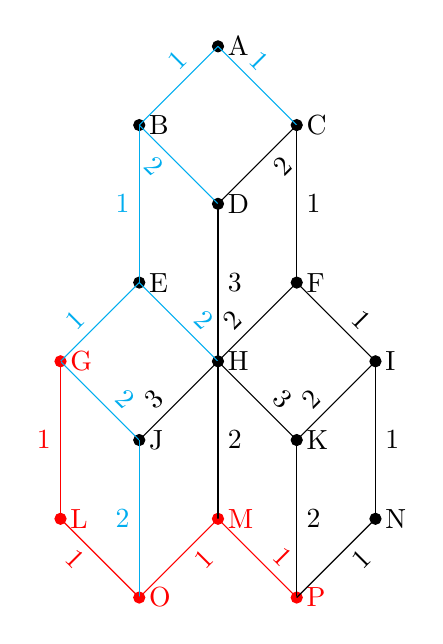
\begin{tikzpicture}[main/.style = {draw, circle}] 
		%Pisteet
		\filldraw[black] (0,6) circle (2pt) node[anchor=west]{A};
		\filldraw[black] (-1,5) circle (2pt) node[anchor=west]{B};
		\filldraw[black] (1,5) circle (2pt) node[anchor=west]{C};
		\filldraw[black] (0,4) circle (2pt) node[anchor=west]{D};
		\filldraw[black] (-1,3) circle (2pt) node[anchor=west]{E};
		\filldraw[black] (1,3) circle (2pt) node[anchor=west]{F};
		\filldraw[red] (-2,2) circle (2pt) node[anchor=west]{G};
		\filldraw[black] (0,2) circle (2pt) node[anchor=west]{H};
		\filldraw[black] (2,2) circle (2pt) node[anchor=west]{I};
		\filldraw[black] (-1,1) circle (2pt) node[anchor=west]{J};
		\filldraw[black] (1,1) circle (2pt) node[anchor=west]{K};
		\filldraw[red] (-2,0) circle (2pt) node[anchor=west]{L};
		\filldraw[red] (0,0) circle (2pt) node[anchor=west]{M};
		\filldraw[black] (2,0) circle (2pt) node[anchor=west]{N};
		\filldraw[red] (-1,-1) circle (2pt) node[anchor=west]{O};
		\filldraw[red] (1,-1) circle (2pt) node[anchor=west]{P};
		% Janat
		\draw [cyan] (0,6) -- node[midway, above left, sloped] {1} (1,5);	% AB
		\draw [cyan] (0,6) -- node[midway, above right, sloped] {1} (-1,5);	% AC
		\draw [cyan] (-1,5) -- node[midway, below left, sloped] {2} (0,4);	% BD
		\draw [cyan] (-1,5) -- node[midway, left] {1} (-1,3);			% BE
		\draw (1,5) -- node[midway, below right, sloped] {2} (0,4);	% CD
		\draw (1,5) -- node[midway, right] {1} (1,3);			% CF
		\draw (0,4) -- node[midway, right] {3} (0,2);			% DH
		\draw [cyan] (-1,3) -- node[midway, above left, sloped] {1} (-2,2);	% EG
		\draw [cyan] (-1,3) -- node[midway, above right, sloped] {2} (0,2);	% EH
		\draw (1,3) -- node[midway, above left, sloped] {2} (0,2);	% FH
		\draw (1,3) -- node[midway, above right, sloped] {1} (2,2);	% FI
		\draw [cyan] (-2,2) -- node[midway, above right, sloped] {2} (-1,1);	% GJ
		\draw [red] (-2,2) -- node[midway, left] {1} (-2,0);			% GL
		\draw (0,2) -- node[midway, above left, sloped] {3} (-1,1);	% HJ
		\draw (0,2) -- node[midway, above right, sloped] {3} (1,1);	% HK
		\draw (0,2) -- node[midway, right] {2} (0,0);			% HM
		\draw (2,2) -- node[midway, above left, sloped] {2} (1,1);	% IK
		\draw (2,2) -- node[midway, right] {1} (2,0);			% IN
		\draw [cyan] (-1,1) -- node[midway, left] {2} (-1,-1);			% JO
		\draw (1,1) -- node[midway, right] {2} (1,-1);			% KP
		\draw [red] (-2,0) -- node[midway, below left, sloped] {1} (-1,-1);	% LO
		\draw [red] (0,0) -- node[midway, below right, sloped] {1} (-1,-1);	% MO
		\draw [red] (0,0) -- node[midway, above right, sloped] {1} (1,-1);	% MP
		\draw (2,0) -- node[midway, below right, sloped] {1} (1,-1);	% NP
		\end{tikzpicture}
		\caption{Dijkstran algoritmi referenssigraafissa.}\label{refDijkstra}
	\end{subfigure}
%	\hfill
	\begin{subfigure}[b]{0.5\textwidth}
		\centering
		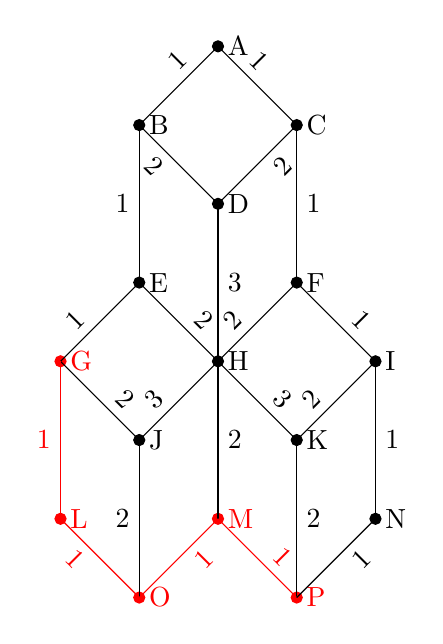
\begin{tikzpicture}[main/.style = {draw, circle}] 
		%Pisteet
		\filldraw[black] (0,6) circle (2pt) node[anchor=west]{A};
		\filldraw[black] (-1,5) circle (2pt) node[anchor=west]{B};
		\filldraw[black] (1,5) circle (2pt) node[anchor=west]{C};
		\filldraw[black] (0,4) circle (2pt) node[anchor=west]{D};
		\filldraw[black] (-1,3) circle (2pt) node[anchor=west]{E};
		\filldraw[black] (1,3) circle (2pt) node[anchor=west]{F};
		\filldraw[red] (-2,2) circle (2pt) node[anchor=west]{G};
		\filldraw[black] (0,2) circle (2pt) node[anchor=west]{H};
		\filldraw[black] (2,2) circle (2pt) node[anchor=west]{I};
		\filldraw[black] (-1,1) circle (2pt) node[anchor=west]{J};
		\filldraw[black] (1,1) circle (2pt) node[anchor=west]{K};
		\filldraw[red] (-2,0) circle (2pt) node[anchor=west]{L};
		\filldraw[red] (0,0) circle (2pt) node[anchor=west]{M};
		\filldraw[black] (2,0) circle (2pt) node[anchor=west]{N};
		\filldraw[red] (-1,-1) circle (2pt) node[anchor=west]{O};
		\filldraw[red] (1,-1) circle (2pt) node[anchor=west]{P};
		% Janat
		\draw (0,6) -- node[midway, above left, sloped] {1} (1,5);	% AB
		\draw (0,6) -- node[midway, above right, sloped] {1} (-1,5);	% AC
		\draw (-1,5) -- node[midway, below left, sloped] {2} (0,4);	% BD
		\draw (-1,5) -- node[midway, left] {1} (-1,3);			% BE
		\draw (1,5) -- node[midway, below right, sloped] {2} (0,4);	% CD
		\draw (1,5) -- node[midway, right] {1} (1,3);			% CF
		\draw (0,4) -- node[midway, right] {3} (0,2);			% DH
		\draw (-1,3) -- node[midway, above left, sloped] {1} (-2,2);	% EG
		\draw (-1,3) -- node[midway, above right, sloped] {2} (0,2);	% EH
		\draw (1,3) -- node[midway, above left, sloped] {2} (0,2);	% FH
		\draw (1,3) -- node[midway, above right, sloped] {1} (2,2);	% FI
		\draw (-2,2) -- node[midway, above right, sloped] {2} (-1,1);	% GJ
		\draw [red] (-2,2) -- node[midway, left] {1} (-2,0);			% GL
		\draw (0,2) -- node[midway, above left, sloped] {3} (-1,1);	% HJ
		\draw (0,2) -- node[midway, above right, sloped] {3} (1,1);	% HK
		\draw (0,2) -- node[midway, right] {2} (0,0);			% HM
		\draw (2,2) -- node[midway, above left, sloped] {2} (1,1);	% IK
		\draw (2,2) -- node[midway, right] {1} (2,0);			% IN
		\draw (-1,1) -- node[midway, left] {2} (-1,-1);			% JO
		\draw (1,1) -- node[midway, right] {2} (1,-1);			% KP
		\draw [red] (-2,0) -- node[midway, below left, sloped] {1} (-1,-1);	% LO
		\draw [red] (0,0) -- node[midway, below right, sloped] {1} (-1,-1);	% MO
		\draw [red] (0,0) -- node[midway, above right, sloped] {1} (1,-1);	% MP
		\draw (2,0) -- node[midway, below right, sloped] {1} (1,-1);	% NP
		\end{tikzpicture}
		\caption{A* referenssigraafissa.}\label{refAStar}
	\end{subfigure}
	\caption{Dijkstran algoritmi ja A* referenssigraafissa.}\label{DijkstraAStarFigs}
\end{figure}

\section{A*-algoritmi}\label{aStar}
A* (luetaan A-tähti tai A-star) on informoitu polunetsintäalgoritmi, joka 
täydentää Dijkstran algoritmia soveltamalla siihen heuristista 
funktiota~\cite{MathewAndMalathy}. Heuristinen funktio on jokin matemaattinen 
funktio, joka palauttaa hinnan, joka mittaa kuinka hyvä tutkittava solmu on 
ongelman ratkaisun kannalta. Kuten Dijkstran algoritmi, myös A* valitsee 
tutkittavakseen halvimmat polut ensin~\cite{DelaunayVoronoiAStar}. Dijkstran 
algoritmissa solmukohdan $n$ läpikäynnin hinnan funktio $F(n)$ on sama kuin 
lähtösolmusta solmulle $n$ johtavan halvimman polun funktio $G(n)$. Siis 
Dijkstran algoritmissa $F(n) = G(n)$ ~\cite{MathewAndMalathy}. Sen sijaan 
A*-algoritmissa yksittäisen solmun $n$ läpikäynnin hinta on 
$F(n) = G(n) + H(n)$, jossa $H(n)$ on heuristisen funktion palauttama arvo 
solmukohdalle $n$ ~\cite{DelaunayVoronoiAStar}. Dijkstran algoritmi voidaan myös 
käsittää A*-algoritmina, jossa $H(n) = 0$ ~\cite{MathewAndMalathy}.\par 
	A*-algoritmin kanssa voidaan käyttää eri heuristisia funktioita 
riippuen siitä, mikä heuristiikka toimii parhaiten tutkittavan ongelman 
kanssa. Tyypillisesti heuristiset funktiot mittaavat käytännössä tutkittavan 
solmun etäisyyttä maalisolmusta tai liikkeen suuntaa~\cite{ProcediaAStar}. 
Tyypillisiä heuristisia funktioita ovat tutkittavan solmun ja maalisolmun 
välinen Manhattan-etäisyys ja Euklidinen etäisyys~\cite{MathewAndMalathy}. 
Manhattan-etäisyys tarkoittaa kahden pisteen $P = (x_1,y_1)$ ja 
$Q = (x_2,y_2)$ välistä etäisyyttä, olettaen liikutaan vain x- ja 
y-akselien suuntaisesti~\cite{MathewAndMalathy}.

\[ d_{Manhattan}(P,Q) =  |x_1 - x_2| + |y_1 - y_2|\]
\par

	Ajetaan \textcite{MathewAndMalathy} perusteella kirjoitetun, 
ohjelmalistauksen \ref{AStarEsim} mukaista A*-algoritmia graafissa 
\ref{refGraf} ja tehdään samat lähtöoletukset kuin aliluvussa \ref{bfs}. 
Käytetään heuristisena funktiona janan pituuden kaavaa

\[ d(P) = \sqrt{(x_G-x_P)^2 + (y_G-y_P)^2} \]

jossa $P$ on $(x,y)$ muotoinen piste, ja G on maalisolmu. Algoritmin ajo 
johtaa kuvan \ref{refAStar} mukaiseen lopputulokseen. Algoritmin löytämä polku 
G-L-O-M-P on sama kuin Dijkstran algoritmin löytämä polku kuvassa 
\ref{refDijkstra}. Tähän päädyttiin kuitenkin huomattavasti nopeammin, koska 
heuristinen funktio ohjasi A*-algoritmia etsimään reittiä oikeasta suunnasta. 
\par
	A* on suosittu algoritmi käytännön sovelluksissa, koska se on 
monipuolinen, helposti toteutettava ja tehokas. Se on useimmiten se algoritmi, 
josta lähdetään liikkeelle kun polunetsintää pitää käytännössä soveltaa 
oikean elämän ongelmiin, esimerkiksi videopelikehityksessä tai 
robotiikassa~\cite{ProcediaAStar}. A* toimii myös pohjana monelle muulle 
algoritmille, koska sitä on helppo muokata ja parannella~\cite{ProcediaAStar}. 
Esimerkiksi D*-algoritmi on A*-algoritmiin perustuva polunetsintäalgoritmi, 
joka on dynaaminen, eli se kykenee reagoimaan etsintäalueen 
muuttumiseen~\cite{applSciLawande}. Hierarkkisen polunetsinnän A* (Hierarchical 
Pathfinding A*, HPA*) on hierarkkiseen polunetsintään kehitetty 
A*-variantti~\cite{applSciLawande}. Lisää hierarkkisesta polunetsinnästä 
aliluvussa \ref{hpa}. \par
	Polunetsintään liittyvissä tieteellisissä tutkimuksissa A* on myös 
suosittu lähtökohta. Usein nämä tutkimukset kehittävät jonkun A* variantin 
johonkin spesifiseen käyttötarkoitukseen~\cite{ProcediaAStar}. Esimerkiksi 
\textcite{MathewAndMalathy} käyttävät tavallista A*-algoritmia, mutta 
kehittävät siihen uudenlaisen heuristisen funktion ja 
\textcite{DelaunayVoronoiAStar} kehittävät A*-pohjaisen polunetsintäalgoritmin 
käytettäväksi robotiikassa.

\section{Hierarkkinen polunetsintä}\label{hpa}
Monet perinteiset polunetsintäalgoritmit skaalautuvat huonosti etsintäalueen 
kasvaessa ja monimutkaistuessa. Esimerkiksi \textcite{rda} demonstroivat 
artikkelissaan, kuinka A*-algoritmi kävi läpi suuren osan etsintäalueesta 
eräässä esimerkkitehtävässä. Tätä varten kehitettiin polunetsintätekniikoita 
suurille etsintäalueille. Yksi tällainen tekniikka on hierarkkinen 
polunetsintä~\cite{rda}. \par
	Hierarkkisessa polunetsinnässä etsintäalue jaetaan pienempiin 
osa-alueisiin, niin että pidetään kirjaa siitä, mitkä osa-alueet ovat 
kytköksissä toisiinsa minkäkin solmujen kautta. Tämän jälkeen 
osa-alueista muodostetaan ylemmän tason graafi~\cite{rda}. Ylemmän tason 
graafista etsitään ensin ylemmän tason polku, joka kertoo minkä 
osa-alueiden kautta varsinainen polku kulkee. Sitten kriittisten osa-alueiden 
läpi etsitään niiden kautta kulkevat polut. Nämä polut yhdistetään lopussa 
varsinaiseksi poluksi. Hierarkkisella polunetsinnällä saadaan 
yksinkertaistettua polunetsintäongelmaa abstraktion avulla ja tämä nopeuttaa 
ratkaisun löytämistä merkittävästi. Näin saadut polut eivät kuitenkaan 
välttämättä ole optimaalisia~\cite{rda}.\par
	Hierarkkisia polunetsintäalgoritmeja on monia erilaisia, esimerkiksi 
hierarkkisen polunetsinnän A* (HPA*) ja navigaatioverkkojen hierarkkisen 
polunetsinnän A* (Hierarchical pathfinding for Navigation Meshes A*, 
HNA*)~\cite{rda}. Hierarkkiset polunetsintäalgoritmit eroavat toisistaan muun 
muassa siinä, että mitä algoritmia käytetään jakamaan etsintäalue ja mitä 
polunetsintäalgoritmia käytetään polkujen löytämiseen. \textcite{rda} 
esittelevät artikkelissaan kehittämänsä alueenlöytöalgoritmin (Regions 
Discovery Algorithm, RDA), jota he vertaavat HPA*-algoritmin 
sisäänrakennettuun tapaan jakaa ruudukkomuotoinen etsintäalue alaruudukoiksi. 
Esimerkkipseudokoodi hierarkkisesta polunetsinnästä löytyy ohjelmalistauksesta 
\ref{HierarkkinenEsim}.
